%!TEX root = ../main.tex


\section{TensorFlow 简介}

\begin{frame}{\secname}
\begin{center}
  \vfill
  \raisebox{-7pt}{
\includegraphics[width = 8cm]{./template/icon_in_cover.pdf}} \scalebox{3.2}{\bfseries 简介}\vspace{10pt}

  \begin{varwidth}{\textwidth}
  \large
  \tableofcontents[sectionstyle = hide/hide, subsectionstyle = show/show/hide]
  \end{varwidth}
  \vfill
\end{center}
\end{frame}

\subsection{TensorFlow 是什么}
\begin{frame}{\insertsection}{\insertsubsection}
    TensorFlow 是一款通过数据流图进行数值计算的开源库. TensorFlow 最早是被 Google Brain 的研究者和工程师开发出来的用于机器学习和深度神经网络的研究. 但是这个系统也同样适用于其他领域.

    TensorFlow 具有很多非常好的特性:%
    %
    \begin{itemize}
        \item \textbf{易用性}, TensorFlow 封装了很多复杂运算, 使用者只需构建计算图.
        \item \textbf{可移植性}, TensorFlow 支持多种平台, 系统以及硬件.
        \item \textbf{自动求导}, TensorFlow 支持自动求导, 给采用基于梯度下降的学习方法带来了极大便利.
        \item \textbf{支持多种语言}, TensorFlow 提供方便易用的 Python 接口, 也支持 C++, Java, Go 等语言.
        \item \textbf{性能最大化}, 可以部署到不同硬件, 并使用线程, 队列, 异步计算来最大化硬件使用效率.
    \end{itemize}
\end{frame}

\subsection{TensorFlow 的主要技术特性}
\begin{frame}{\insertsection}{\insertsubsection}
    \begin{table}[!htb]
        \centering
        \begin{tabu}{X[l, -1]|X[l]}
            \tabucline[1pt]{-}
            编程模型 & Dataflow-Like Model\\\hline
            语言     & Python, C++, Go, Rust, Haskell, Java, Julia, JavaScript, R\\\hline
            部署     & Code-once, run everywhere\\\hline
            计算资源 & CPU, GPU, TPU\\\hline
            实现方式 & Local Implementation, Distributed Implementation\\\hline
            平台支持 & Google Cloud Platform, Hadoop File System\\\hline
            数学表达 & Math Graph Expression, Auto Differentiation\\\hline
            优化     & Common Subexpression Elimination,\\
                     & Asynchronous Kernel Optimization,\\
                     & Communication Optimization,\\
                     & Model Parallelism, Data Parallelism, Pipeline\\
            \tabucline[1pt]{-}
        \end{tabu}
    \end{table}
\end{frame}


% \begin{frame}{\insertsection}{TensorFlow 的工作原理}
%     \begin{minipage}[m]{0.5\textwidth}
%     TensorFlow 是用数据流图对计算过程进行描述的. 在数据流图中, 节点通常代表数学运算, 边表示节点之间的某种联系, 边负责在节点之间传输多维数据, 即 Tensor.

%     节点可以被分配到多个计算设备上, 可以异步和并行的进行操作. 因为是有向图, 所以只能等待之前的节点运行结束, 当前节点才能执行操作. 如图所示是一个简单的计算流图, 且它的表达式为%
%     \[
%         \bigg(2.2 - \Big(\frac{x}{11}\Big)\bigg) + \big(7 \times \cos(y)\big)\text{.}
%     \]
%     \end{minipage}\hfill
%     \begin{minipage}[m]{0.4\textwidth}
%     \begin{figure}[!htb]
%         \centering
%         \scalebox{0.8}{%!TEX root = ../main.tex

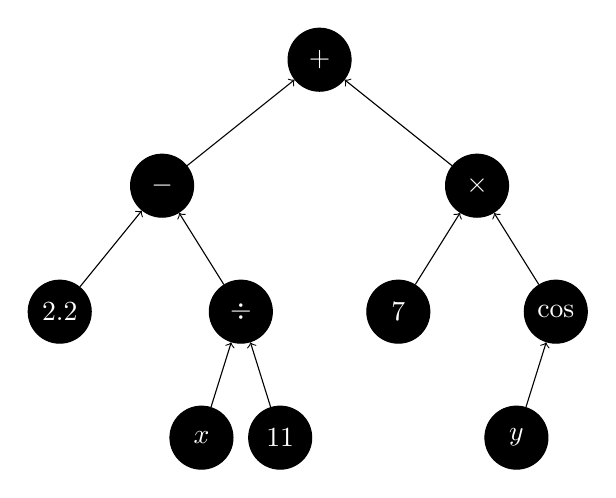
\begin{tikzpicture}[%
    node/.style = {circle, draw, minimum size = 0.8cm, align = flush center, inner sep = 0pt, fill = black, text = white},
    y = 0.8cm]

    \node[node] (x) at (5, 0) {$x$};
    \node[node] (11) at (6, 0) {$11$};
    \node[node] (y) at (9, 0) {$y$};
    \node[node] (div) at (5.5, 2) {$\div$};
    \node[node] (22) at (3.2, 2) {$2.2$};
    \node[node] (7) at (7.5, 2) {$7$};
    \node[node] (cos) at (9.5, 2) {$\cos$};
    \node[node] (sub) at (4.5, 4) {$-$};
    \node[node] (times) at (8.5, 4) {$\times$};
    \node[node] (plus) at (6.5, 6) {$+$};

    \draw[->] (x) -- (div);
    \draw[->] (11) -- (div);
    \draw[->] (y) -- (cos);
    \draw[->] (22) -- (sub);
    \draw[->] (div) -- (sub);
    \draw[->] (7) -- (times);
    \draw[->] (cos) -- (times);
    \draw[->] (sub) -- (plus);
    \draw[->] (times) -- (plus);
\end{tikzpicture}
}
%     \end{figure}
%     \end{minipage}
% \end{frame}
